\documentclass[14pt, letterpaper, twoside]{article}
\usepackage[hmarginratio=1:1, margin=1in]{geometry}
\usepackage{fancyhdr}
\usepackage{titlepic}
\usepackage{pdfpages}
\usepackage[colorlinks=true, urlcolor=blue, linkcolor=blue]{hyperref}
\usepackage{graphicx}
\usepackage[mmddyyyy]{datetime}
\usepackage{fancyhdr}
\setlength{\parskip}{2mm}
\setlength{\parindent}{0mm}
\setcounter{secnumdepth}{3}
\setcounter{tocdepth}{10}
\usepackage{setspace}
\usepackage{times}

\titlepic{
\includegraphics[width=2in]{logo.png}}
\title{\textbf{What's Our Name?}
	\begin{spacing}{1.5}
	This activity accomplishes the goal of creating a class name as well as naming our table teams in our classrom. It also imparts valuable life skills,
	character development, and a strong sense of belonging and unity within the school community. It encourages students to become active participants in
	shaping their class and  school's identity and culture, emphasizing the importance of self-discipline, teamwork, and leadership.
	\end{spacing}}
		\date{}
\author{September 11, 2023}

% Cover Page
%%%%%%%%%%%%%%%%%%%%%%%%%%%%%%%%%%%%%%%%%%%%%%%%%%%%%%%%%%%%%%%%%%%%%%%%%%%%%%%%%%%%%%%%%%%%%%%%%%%%%%%%%%%%%%%%%%%%%%%%%%%%%%%%%%%%%%%%%%%%%%%%%%%%%%%%%
\begin{document}
	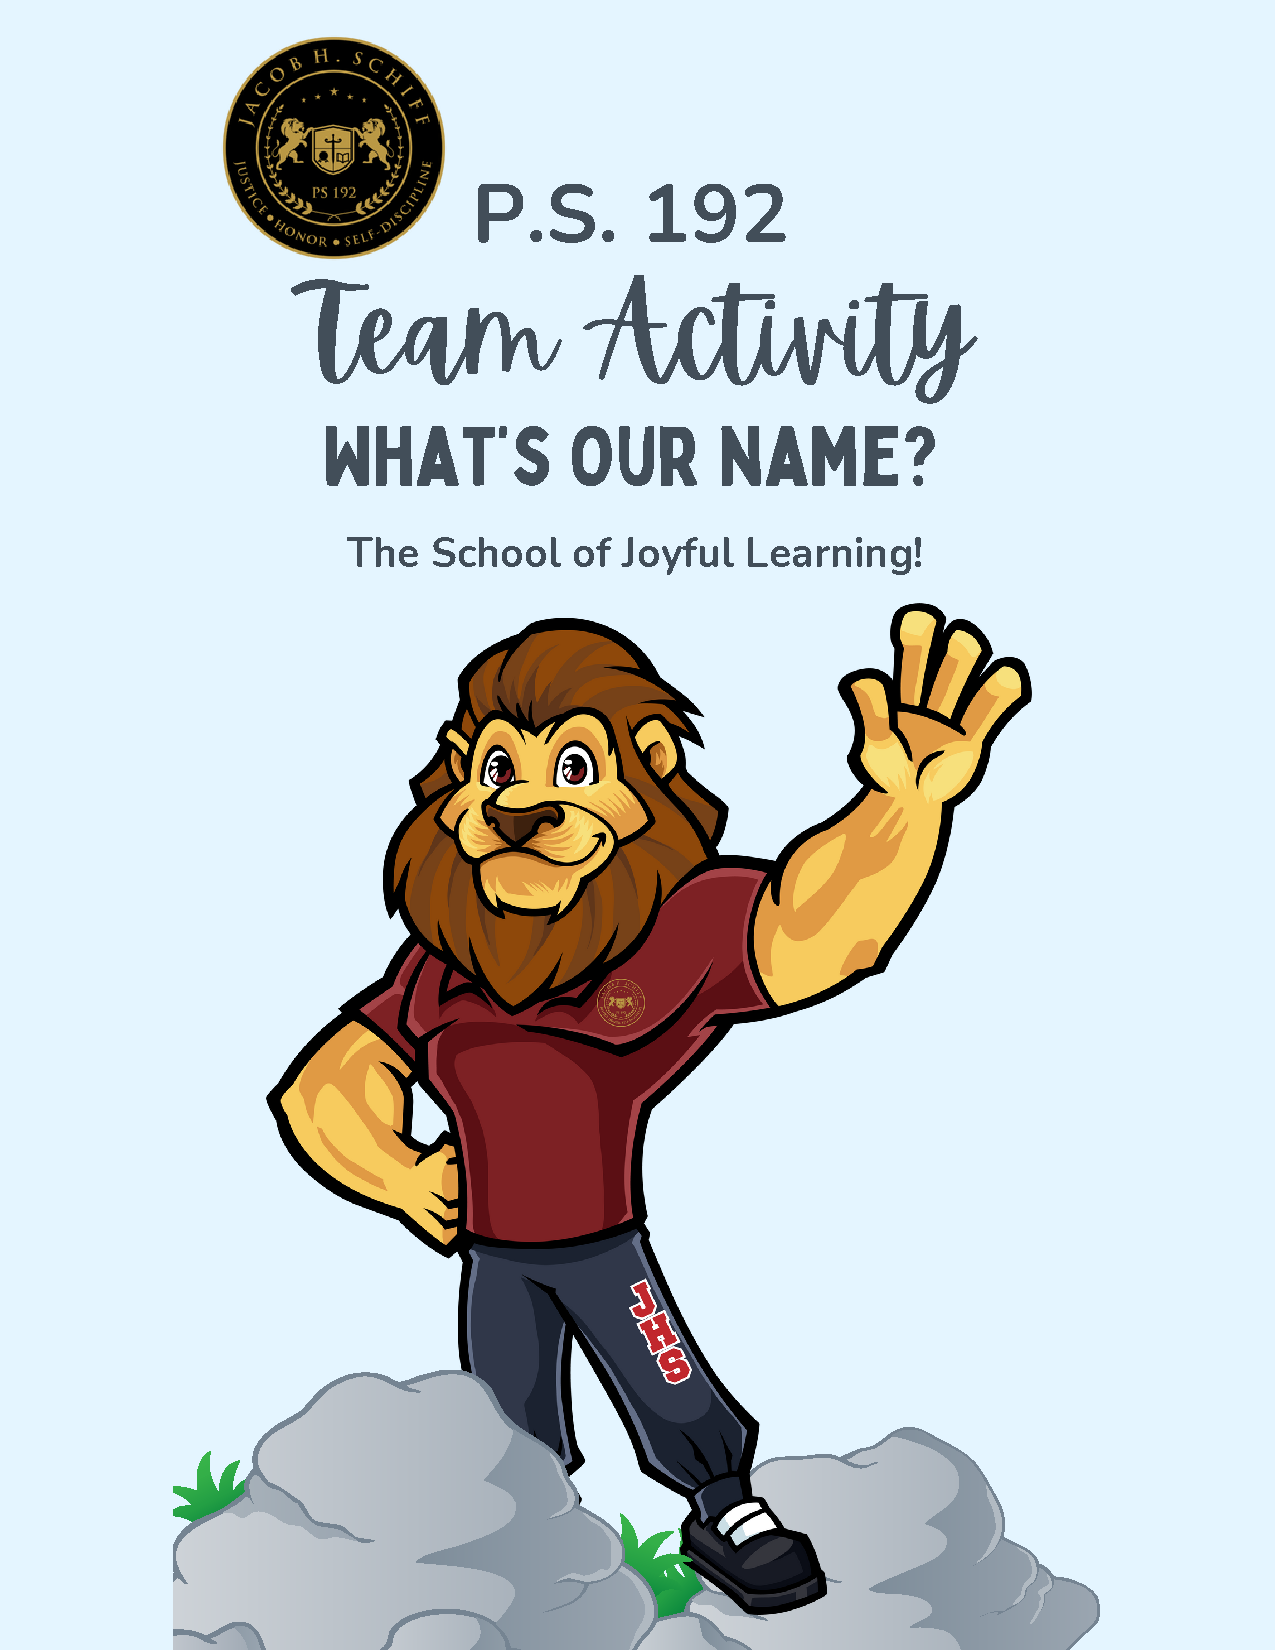
\includepdf[pages=1,fitpaper]{ps192-mascot}
		\begin{titlepage}
		\maketitle
		\thispagestyle{empty}
		\end{titlepage}
	\pagenumbering{arabic}
	\pagestyle{headings}
	\fancyhf{}
	\fancyhead[L]{\textit{Name Our Class and Table Teams}}
	\fancyhead[R]{\thepage}
	\fancyfoot[C]{The School of Joyful Learning!}
	\pagestyle{fancy}
	\renewcommand{\footrulewidth}{1 px}
% TOC
%%%%%%%%%%%%%%%%%%%%%%%%%%%%%%%%%%%%%%%%%%%%%%%%%%%%%%%%%%%%%%%%%%%%%%%%%%%%%%%%%%%%%%%%%%%%%%%%%%%%%%%%%%%%%%%%%%%%%%%%%%%%%%%%%%%%%%%%%%%%%%%%%%%%%%%%%
	\newpage
	\tableofcontents
	\thispagestyle{empty}
	\newpage

\section{Activity Description}
"What's Our Name?" is an engaging and educational activity designed for emphasizing and reinforcing the school's core values of justice, honor, and self-discipline. In addition, this, the activity fosters a sense of belonging, collaboration, and leadership within the class and school community.
	\subsection{What Kids Will Learn:}
		\begin{itemize}
		\item What Kids Will Learn:
			\begin{itemize}
			\item Core Values: 
				\begin{itemize}
				\item Students will gain a deeper understanding of the school's core values—justice, honor, and self-discipline—through discussions and 						brainstorming sessions. They will learn to connect these values with real-life examples and how they shape our school's culture.
				\end{itemize}
			\item Creativity and Collaboration:
				\begin{itemize}
				\item The activity encourages students to work together in groups to brainstorm and propose names for their class and table team. They 						will learn to combine their creative ideas, compromise, and make collective decisions, promoting teamwork and collaboration. Explicitly 						model, rehearse the K-2 or 3-5 Collaborative Discussion guide and the protocol for working in groups.
				\end{itemize}
			\item Communication Skills:
				\begin{itemize}
				\item When presenting their chosen team name to the class, students will develop their communication skills by articulating their ideas 						and explaining how the names relate to them and the school's values. This helps improve their ability to express themselves clearly and 						persuasively. Explicitly model and rehearse the K-2 or 3-5 Discussion guide and the TAG protocol for sharing.
				\end{itemize}
			\item Democracy and Voting: Voting to Select a Name for the Class
				\begin{itemize}
				\item The voting process teaches students about democratic decision-making. They will experience the importance of individual voices and 						the collective will of the community in choosing a class name.
				\end{itemize}
			\item Leadership Principles:
				\begin{itemize}
				\item During the leadership discussion, students will explore the qualities and responsibilities of leaders in promoting unity and 							collaboration. They will understand that leadership isn't limited to individuals but can be collective and inclusive.
				\end{itemize}
			\item Sense of Belonging:
				\begin{itemize}
				\item Through this activity students develop a sense of belonging and ownership in their school community.
				\end{itemize}
			\item Symbolism:
				\begin{itemize}
				\item Students will learn about symbolism and its role in representing their class and team's identity. They will see how the chosen name 						can inspire pride and a strong sense of belonging and identity among students.
				\end{itemize}
			\item Long-Term Engagement:
				\begin{itemize}
				\item The ongoing implementation of the class and table team name in school activities will reinforce the values and sense of community 						established during the activity, ensuring that these lessons are carried forward throughout the school year.
				\end{itemize}
			\end{itemize}
	\end{itemize}
	\newpage

\section{Title: "Name Our Class and Table Teams"}
	\subsection{Lesson Objective:}
	
	The objective of this educational activity is to engage our students in a 		collaborative and creative process to name our school's lion mascot. Through 	this activity, students will not only learn about the school values of 			justice, honor, and self-discipline but also develop a sense of unity, 			collaboration, and 	leadership within our school community. Read aloud and 		analyze the objective of the lesson, and co-create the I can statement with 		students.
	
	Standards:
	
	CASEL 13: Relationship Skills: Learners will be able to use active listening 	and assertive, clear communication when expressing thoughts and ideas.
	
	CASEL 16: Relationship Skills:Learners will be able to work cooperatively 		and productively in a group and overcome setbacks and disagreements.				\begin{itemize}
		\item Materials Needed:
			\begin{itemize}
    		\item Coloring materials (crayons, colored pencils, markers)
    		\item Large poster paper
    		\item Sticky notes or index cards
    		\item Ditigital and audible countdown clock
    		\item Computer and projector (optional)
    		\item Prize for the winning name (e.g.,certificate, Lunch with the 				Pricipal and teacher, 1 period of recess)
    		\end{itemize}
    	\item Activity Steps:
    		\begin{itemize}
    		\item Introduction (10 minutes):
    		
    		Begin by gathering all the students in the area(sitting in a 						circular or "U" shape. Explain the purpose of the activity to name 				the class and each team. Emphasize that the chosen name should 					reflect the school's core values of justice, honor, and self-						discipline. Discuss the importance of unity, collaboration, and 					leadership 	within the school community. Explicitly model, discuss 				and rehearse the the role of the speaker and the role of the 						listener. Co-create the anchor chart or reference it, if already					created.
    	\item Brainstorming (15 minutes):
    		\begin{itemize}
    		\item Break the students into groups ( 4-6 students), ensuring that 				each group has a mix of levels and personalities to encourage 					collaboration. Give each group a large sheet of poster paper and 					markers. Ask them to brainstorm names that align with the school 					values. Encourage creativity and teamwork.Teacher is canvasing the 				room to document individual and team trends and patterns of the 					teams. Use the discussion guide (role of the speaker/listener) to 				anchored your noticings. Record noticings.
    		\end{itemize}
    	\item Presentations (20 minutes):
    		\begin{itemize}
    		\item Each group will present their chosen class and table team name 			and explain why and how it reflects our core values. Use chart paper 			or a google doc to write down the names as they are presented. 					Discuss the qualities of each proposed name and how it relates to 				the school's values.
    		\end{itemize}
    	\item Voting (10 minutes):
    		\begin{itemize}
    		\item Give each student sticky notes or index cards and ask them to 				vote for their favorite class name from the presented options. They 				can write the name on the card or stick the sticky note next to the 				name on the board.
    		\end{itemize}
    	\item Lesson Wrap-Up: Leadership Discussion (10 minutes):
		\begin{itemize}
    		\item While the votes are being counted, lead a discussion about leadership and how leaders can inspire unity and collaboration. Emphasize the role of the speaker and the role of the listener. Based on your observations, co-create a T-chart to create a list "The Criteria We mastered" and "The Criteria We Need to Work on as a Team" when working in collaborative learning groups.
    		\end{itemize}
    		\item Announcement of the Winning Name (5 minutes):
		\begin{itemize}
    		\item Announce the winning class name that received the most votes. This is the name that will be displayed on your class door and used	by all members of the class. Share the class name and the table team names with the clusters and service providers to ensure alignment accross the school. 
    		\end{itemize}
		\item Name Implementation (ongoing):
		\begin{itemize}
    		\item Application of objective learned: Incorporate the newly chosen class name and table team names into class activities and events, reinforcing the values of justice, honor, and self-discipline, as well as the sense of unity and collaboration among students. 
    		\end{itemize}
    		
Teacher Final Summary: Draft a summary in chart paper to model a lesson reflection in the class reflection log previously created during the name the mascot activity. 
"Today we learned not only to use our creativity but also learned importance of working together to accomplish a common goal." Provide 2-3 evidence from the T-chart to draft the summary using RACE (grades 3-5) or RADD (grades K-2). These summaries will be use as relection exemplars for you to discuss and co-create the criteria for "What Makes a Good Lesson Reflection."
		\end{itemize}
    
	\end{itemize}

\end{document}
